\vspace{1em}
\scalebox{0.85}{
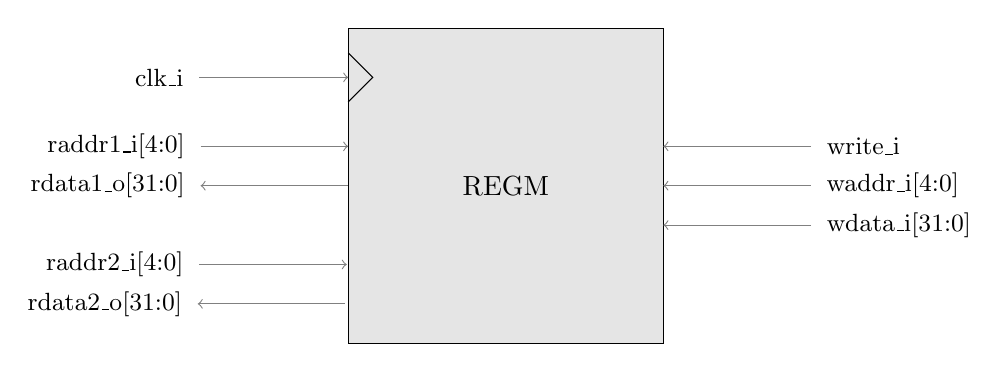
\begin{tikzpicture}[scale=1.25, draw=gray, inner sep=0, outer sep=0]
  \node[rectangle, draw=black,
    align=center,
    minimum height = 4cm,
    minimum width = 4cm,
    fill = gray!20] (block) at (0, 0) {REGM};

  \node (lport2) at ([yshift=0cm]block.west) {};
  \node (lport1) at ([yshift=0.4cm]lport2.center) {};
  \draw[->] ([xshift=-1.5cm]lport1.center) node[left=0.2cm, anchor=east]{\small raddr1\_i[4:0]} -- (lport1.center);
  \draw[<-] ([xshift=-1.5cm]lport2.center) node[left=0.2cm, anchor=east]{\small rdata1\_o[31:0]} -- (lport2.center);

  \node (lport3) at ([yshift=-0.8cm]lport2.west) {};
  \node (lport4) at ([yshift=-0.4cm]lport3.west) {};
  \draw[->] ([xshift=-1.5cm]lport3.center) node[left=0.2cm, anchor=east]{\small raddr2\_i[4:0]} -- (lport3.center);
  \draw[<-] ([xshift=-1.5cm]lport4.center) node[left=0.2cm, anchor=east]{\small rdata2\_o[31:0]} -- (lport4.center);

  \node (rport2) at (block.east) {};
  \node (rport1) at ([yshift=0.4cm]rport2.center) {};
  \node (rport3) at ([yshift=-0.4cm]rport2.center) {};
  \draw[->] ([xshift=1.5cm]rport1.center) node[right=0.2cm, anchor=west]{\small write\_i} -- (rport1.center);
  \draw[->] ([xshift=1.5cm]rport2.center) node[right=0.2cm, anchor=west]{\small waddr\_i[4:0]} -- (rport2.center);
  \draw[->] ([xshift=1.5cm]rport3.center) node[right=0.2cm, anchor=west]{\small wdata\_i[31:0]} -- (rport3.center);

  \node (clk) at ([yshift=-0.5cm]block.north west) {};
  \draw[->] ([xshift=-1.5cm]lport3.center |- clk.center) node[left=0.2cm, anchor=east]{\small clk\_i} -- (clk.center);
  % clk triangle
  \draw[-, draw=black] ([yshift=0.25cm]clk.center) -- ([xshift=0.25cm]clk.center) -- ([yshift=-0.25cm]clk.center);
\end{tikzpicture}
}
